\documentclass{article}

\usepackage{graphicx}
\usepackage{tikz}
\usepackage{tikzsymbols}
\usetikzlibrary{calc,patterns,shapes.geometric}
\pagestyle{empty}
\usepackage[margin=0pt]{geometry}
\geometry{papersize={14in,12in}}

\def\centerarc[#1](#2)(#3:#4:#5){\draw[#1] ($(#2)+({#5*cos(#3)},{#5*sin(#3)})$) arc (#3:#4:#5);}

\begin{document}
	\begin{figure}
		\centering
		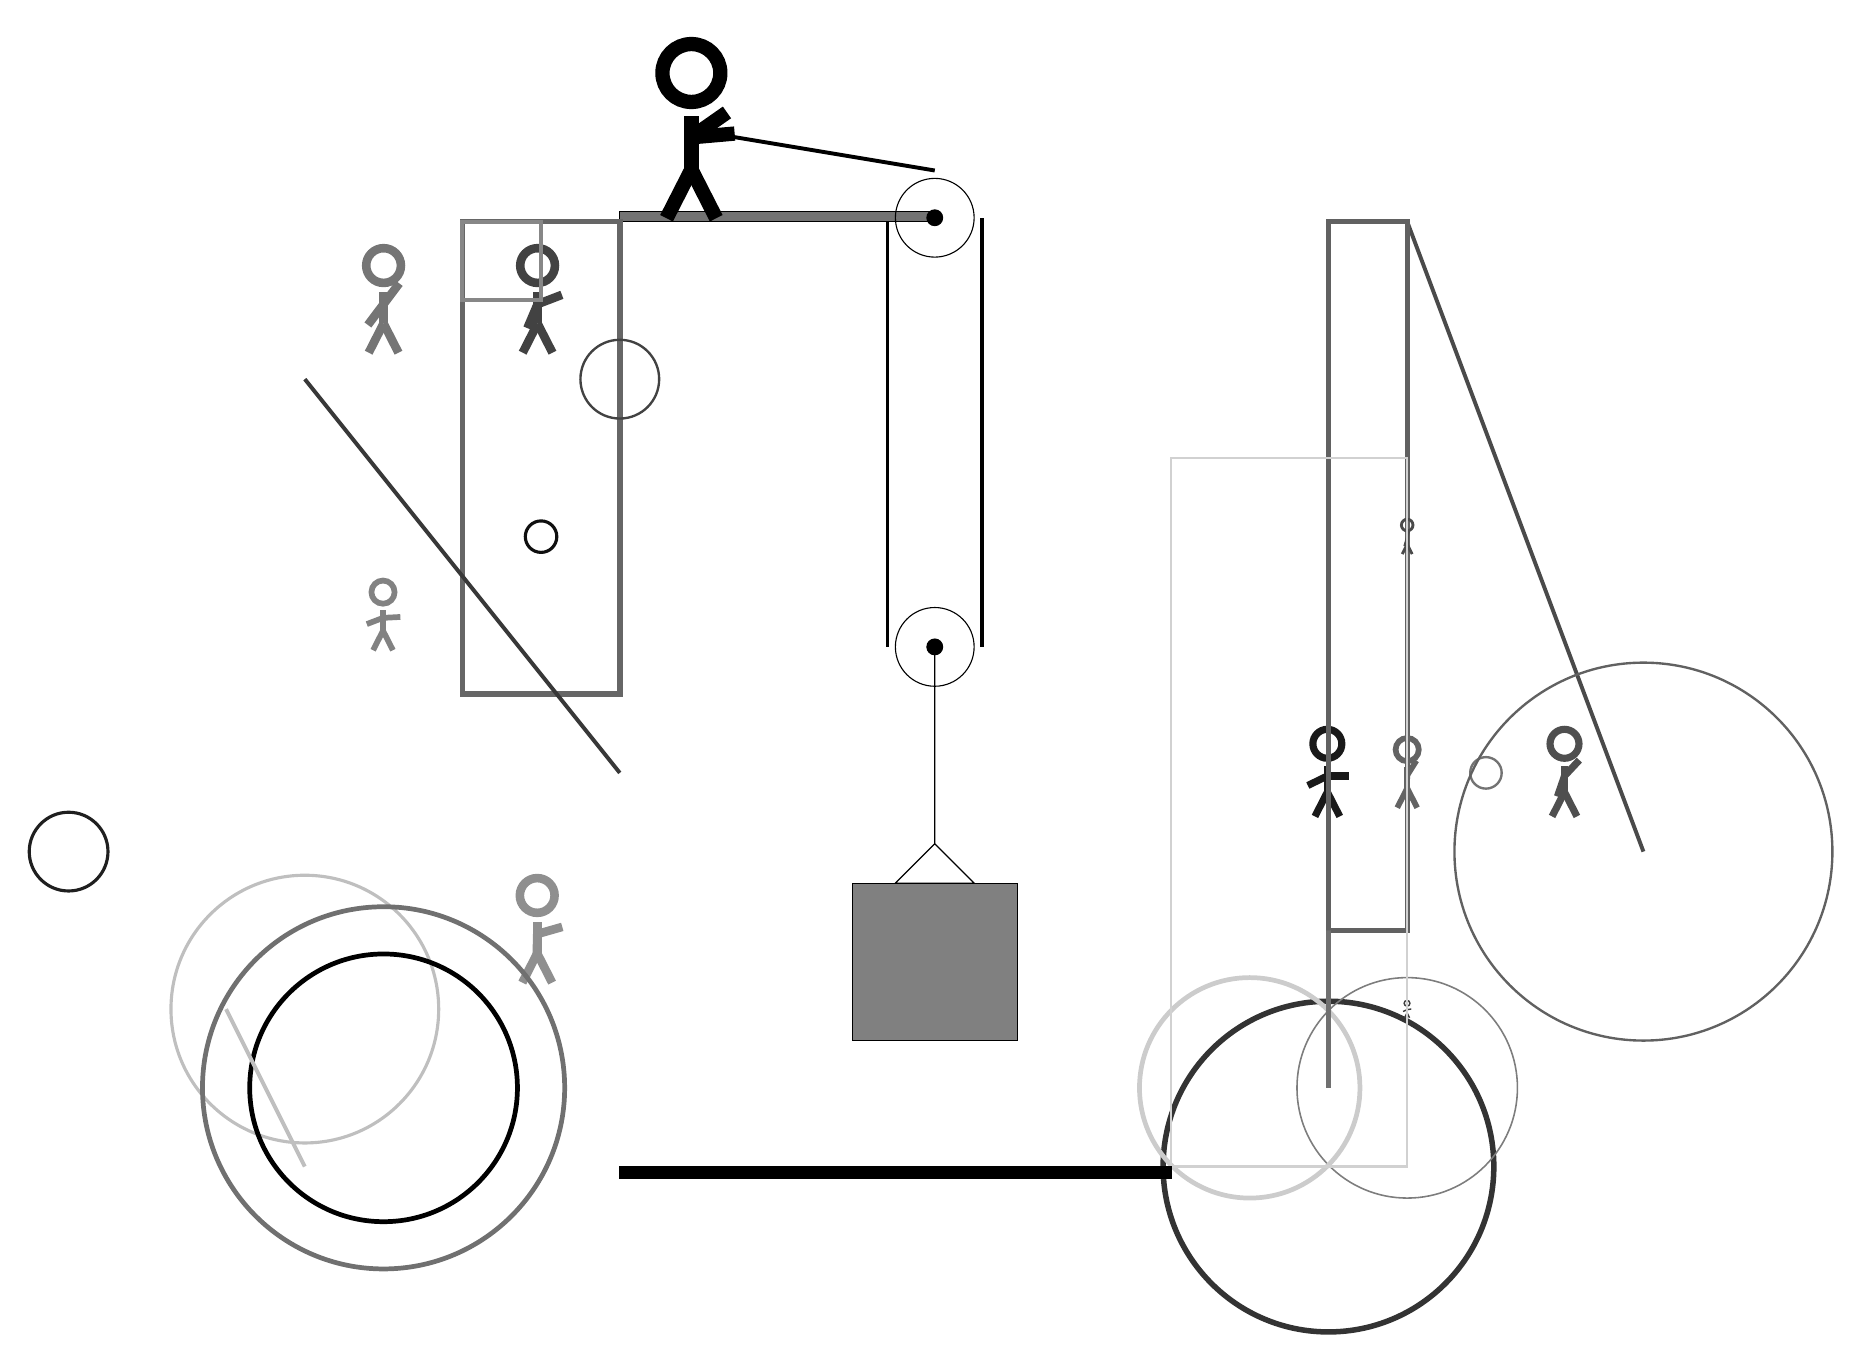
\begin{tikzpicture}
			%%%%% START %%%%%
			
			\draw[fill=black!55] (-2, 9) rectangle (2, 9.125);
			
			\draw (2, 3.6) circle (0.5);
			\draw[fill=black] (2, 3.6) circle (0.1);
			
			\draw (2, 9.05) circle (0.5);
			\draw[fill=black] (2, 9.05) circle (0.1);
			
			\draw (2, 3.6) -- (2, 1.1) -- (1.5, 0.6) -- (2.5, 0.6) -- (2, 1.1);
			\draw[fill=black!50] (0.95, 0.6) rectangle (3.05, -1.4);
			
			\draw[line width=0.5mm] (1.4, 9) -- (1.4, 3.6);
			\centerarc[line width=0.5mm](2, 3.6)(180:360:0.6);
			\draw[line width=0.5mm](2.6, 3.6) -- (2.6, 9.05);
			\centerarc[line width=0.5mm](2, 9.05)(0:90:0.6);
			\draw[line width=0.5mm](2, 9.65) -- (-1, 10.15);
			
			\node at (-1, 10.15) {\Strichmaxerl[10][-175][35]};
			
			\draw [line width=0.4mm, color=black!94](-3, 5) circle (0.2);
			
			\draw[line width=0.7mm, color=black!60] (-2, 3) rectangle (-4, 9);
			\draw [line width=0.3mm, color=black!55](9, 2) circle (0.2);
			\node[line width=0.2mm, color=black!49] at (-5, 4) {\Strichmaxerl[4][21][3]};
			
			\draw [line width=0.7mm, color=black!80](7, -3) circle (2.1);
			\draw [line width=0.4mm, color=black!25](-6, -1) circle (1.7);
			\draw[line width=0.5mm, color=black!71](8, 9) -- (11, 1);
			
			\node[line width=0.3mm, color=black!90] at (7, 2) {\Strichmaxerl[5][26][0]};
			\draw[line width=0.6mm, color=black!62] (7, 9) rectangle (8, 0);
			
			\draw [line width=0.2mm, color=black!51](8, -2) circle (1.4);
			
			\node[line width=0.4mm, color=black!54] at (-5, 8) {\Strichmaxerl[6][53][53]};
			\draw [line width=0.4mm, color=black!88](-9, 1) circle (0.5);
			\draw [line width=0.6mm, color=black!20](6, -2) circle (1.4);
			
			\node[line width=0.4mm, color=black!61] at (8, 2) {\Strichmaxerl[4][89][58]};
			\draw[line width=0.7mm, color=black!56] (7, 0) rectangle (7, -2);
			\node[line width=0.2mm, color=black!69] at (10, 2) {\Strichmaxerl[5][71][47]};
			\draw [line width=0.3mm, color=black!62](11, 1) circle (2.4);
			
			\draw[line width=0.5mm, color=black!78](-2, 2) -- (-6, 7);
			\draw [line width=0.6mm, color=black!100](-5, -2) circle (1.7);
			\node[line width=0.7mm, color=black!44] at (-3, 0) {\Strichmaxerl[6][89][16]};
			\draw [line width=0.3mm, color=black!74](-2, 7) circle (0.5);
			\draw [line width=0.6mm, color=black!56](-5, -2) circle (2.3);
			
			\draw[line width=0.5mm, color=black!25](-7, -1) -- (-6, -3);
			\node[line width=0.5mm, color=black!71] at (8, 5) {\Strichmaxerl[2][74][78]};
			\node[line width=0.2mm, color=black!74] at (-3, 8) {\Strichmaxerl[6][67][21]};
			
			\node[line width=0.5mm, color=black!76] at (8, -1) {\Strichmaxerl[1][24][10]};
			\draw[line width=0.5mm, color=black!47] (-4, 9) rectangle (-3, 8);
			\draw[line width=0.3mm, color=black!18] (5, -3) rectangle (8, 6);
			
			
			\draw[fill=black] (-2, -3) rectangle (5, -3.15);
			
			%%%%% END %%%%%
		\end{tikzpicture}
	\end{figure}	
\end{document}